\documentclass[oneside,fleqn,11pt]{book}
\usepackage[a4paper, total={7.2in, 10.3in}]{geometry}
\usepackage{tikz}
\usetikzlibrary{calc}
\usepackage{setspace}
\usepackage{graphicx}
\usepackage{amsmath}
\usepackage{amssymb}
\DeclareMathOperator\dx{\mathrm{d}\mathit{x}}
\DeclareMathOperator\cis{cis}
\DeclareMathOperator\sech{sech}
\DeclareMathOperator\csch{csch}
\DeclareMathOperator\arsinh{arsinh}
\DeclareMathOperator\arcosh{arcosh}
\DeclareMathOperator\artanh{artanh}
\DeclareMathOperator\cosec{cosec}
\DeclareMathOperator\Nset{\mathbb{N}}
\DeclareMathOperator\Zset{\mathbb{Z}}
\DeclareMathOperator\Qset{\mathbb{Q}}
\DeclareMathOperator\Rset{\mathbb{R}}
\DeclareMathOperator\Iset{\mathbb{I}}
\DeclareMathOperator\Cset{\mathbb{C}}

\usepackage{pgfplots}
\graphicspath{ {./images/} }
\usepackage{bookmark}
\setcounter{tocdepth}{0}
\usepackage{import}
\usepackage{mathtools}

\makeatletter
\g@addto@macro\bfseries{\boldmath}
\makeatother

\DeclarePairedDelimiter{\ceil}{\lceil}{\rceil}
\hypersetup{
	colorlinks   = true, %Colours links instead of ugly boxes
	urlcolor     = blue, %Colour for external hyperlinks
	linkcolor    = black, %Colour of internal links
	citecolor   = red %Colour of citations
}

\newcommand{\tikzAngleOfLine}{\tikz@AngleOfLine}
\def\tikz@AngleOfLine(#1)(#2)#3{%
	\pgfmathanglebetweenpoints{%
		\pgfpointanchor{#1}{center}}{%
		\pgfpointanchor{#2}{center}}
	\pgfmathsetmacro{#3}{\pgfmathresult}%
}

% math font
\usepackage{amsmath}
\usepackage{amssymb}
\usepackage{amsthm}
\usepackage{mathtools}
%\usepackage{arev}

% color
\usepackage[table]{xcolor}

\usepackage[many]{tcolorbox}
\usepackage{pifont}
\usepackage{hyperref}
\usepackage{blindtext}
\counterwithin*{chapter}{part}
\newcommand*{\Part}[2][\partheading]{%
  \refstepcounter{part}%
  \def\partheading{#2}%
  \part*{#2}%
  \addcontentsline{toc}{part}{#1}%
}
% \hypersetup{%
% 	linktoc=all,%
% 	bookmarksnumbered,%
% 	bookmarksopen,%
% 	hidelinks}
% \usepackage{bookmark}
% \bookmarksetup{
% 	addtohook={%
% 		\ifnum\bookmarkget{level}=0%
% 		\bookmarksetup{color=red}%
% 		\fi%
% 		\ifnum\bookmarkget{level}=1%
% 		\bookmarksetup{color=blue}%
% 		\fi%
% 		\ifnum\bookmarkget{level}=2%
% 		\bookmarksetup{color=teal}%
% 		\fi}}
% % enumerate
\usepackage[inline]{enumitem}
\usepackage{multicol}
\usepackage[inline]{enumitem}
\usepackage{tasks}
\usepackage{caption}
\usepackage{subcaption}
\usepackage{cancel}

\renewcommand\rmdefault{ptm}
\renewcommand\sfdefault{ptm}

\tcbset{
	colframe=magenta,
	colback=magenta!12!white,
	boxed title style={colback=magenta},
	breakable,
	enhanced,
	sharp corners,
	boxsep=1pt,
	attach boxed title to top left={yshift=-\tcboxedtitleheight,  yshifttext=-.75\baselineskip},
	boxed title style={boxsep=1pt,sharp corners},
	fonttitle=\bfseries\sffamily,
	drop lifted shadow
}
\newtcolorbox{solution}[1][]{
	no shadow,
	top=2ex,
	boxrule=0pt,
	leftrule=1.4pt,
	title={Solution},
	colframe=green!79!blue,
	colback=green!12!white,
	boxed title style={colback=green!79!blue},
	overlay unbroken and first={
		\node[below right,font=\small,color=magenta,text width=.8\linewidth]
		at (title.north east) {#1};
	}
}
\newtcolorbox[auto counter,number within=chapter,number format=\arabic]{activity}[1][]{
	title={Activity~\thetcbcounter},
	colframe=green,
	colback=green!22!white,
	coltitle=black,
	boxed title style={colback=green},
	overlay unbroken and first={
		\node[below right,font=\small,color=green,text width=.8\linewidth]
		at (title.north east) {#1};
	}
}
\newtcolorbox[auto counter,number within=chapter,number format=\arabic]{definition}[1][]{
	title={Definition~\thetcbcounter},
	colframe=blue,
	colback=blue!12!white,
	boxed title style={colback=blue},
	overlay unbroken and first={
		\node[below right,font=\small,color=blue,text width=.8\linewidth]
		at (title.north east) {#1};
	}
}
\newtcolorbox[auto counter,number within=chapter,number format=\arabic]{theorem}[1][]{
	title={Theorem~\thetcbcounter},
	colframe=violet,
	colback=violet!12!white,
	fontupper=\itshape,
	boxed title style={colback=violet},
	overlay unbroken and first={
		\node[below right,font=\small,color=violet,text width=.8\linewidth]
		at (title.north east) {#1};
	}
}
\newtcolorbox[auto counter,number within=chapter,number format=\arabic]{example}[1][]{
	title={Example~\thetcbcounter},
	colframe=magenta,
	colback=magenta!12!white,
	boxed title style={colback=magenta},
	overlay unbroken and first={
		\node[below right,font=\small,color=magenta,text width=.8\linewidth]
		at (title.north east) {#1};
	}
}
\newtcolorbox[auto counter,number within=chapter,number format=\arabic]{exercise}[1][]{
	title={Exercise~\thetcbcounter},
	colframe=red,
	colback=red!12!white,
	boxed title style={colback=red},
	overlay unbroken and first={
		\node[below right,font=\small,color=red,text width=.8\linewidth]
		at (title.north east) {#1};
	}
}
\newtcolorbox[auto counter,number within=chapter,number format=\arabic]{generality}[1][]{
	title={Generality~\thetcbcounter},
	colframe=teal,
	colback=teal!12!white,
	boxed title style={colback=teal},
	overlay unbroken and first={
		\node[below right,font=\small,color=teal,text width=.8\linewidth]
		at (title.north east) {#1};
	}
}
\newtcolorbox[auto counter,number within=chapter,number format=\arabic]{property}[1][]{
	title={Property~\thetcbcounter},
	colframe=teal,
	colback=teal!12!white,
	boxed title style={colback=teal},
	overlay unbroken and first={
		\node[below right,font=\small,color=teal,text width=.8\linewidth]
		at (title.north east) {#1};
	}
}
\newtcolorbox{remark}[1][]{
	title={\scalebox{1.75}{\raisebox{-.25ex}{\ding{43}}}~Remark},
	colframe=yellow!45!white,
	colback=yellow!45!white,
	coltitle=violet,
	fontupper=\sffamily,
	boxed title style={colback=yellow!45!white},
	boxed title style={boxsep=1ex,sharp corners},%%
	overlay unbroken and first={
		\node[below right,font=\normalsize,color=red,text width=.8\linewidth]
		at (title.north east) {#1};
	}
}
\newtcolorbox{note}[1][]{
	title={\scalebox{1.75}{\raisebox{-0.25ex}{\ding{45}}}~Note},
	colframe=yellow!45!white,
	colback=yellow!45!white,
	coltitle=violet,
	fonttitle=\bfseries\sffamily,
	fontupper=\sffamily,
	boxed title style={colback=yellow!45!white},
	boxed title style={boxsep=1ex,sharp corners},%%
	overlay unbroken and first={
		\node[below right,font=\normalsize,color=red,text width=.8\linewidth]
		at (title.north east) {#1};
	}
}

\makeatletter
\g@addto@macro\bfseries{\boldmath}
\makeatother

\title{A Level Mathematics Notes - Pure Mathematics}
\author{Xingzhi Lu}
\date{}

\begin{document}
\everymath{\displaystyle}
\maketitle
\tableofcontents

\part{Pure 1 Contents}
\chapter{Algebraic expressions}
\section{Indices calculations}
\begin{itemize}
    \item $a^m \times a^n = a^{m+n}$
    \item $a^m \div a^n = a^{m-n}$
    \item $(a^m)^n = a^{mn}$
    \item $a^{\frac{m}{n}} = \sqrt[n]{a^m}$
\end{itemize}

\section{Surds}
\subsection{Rationalising the denominator}
Multiply both the numerator and the denominator by the conjugate of the denominator

\chapter{Quadratics}
\section{Maclaurin series}
$$f(x)=f(0)+f'(0)x+\frac{f''(0)x^2}{2!}+\dots+\frac{f^{(r)}(0)x^r}{r!}+\dots$$
This series is valid provided that $f(0), f'(0), f''(0),\dots,f^{(r)}(0),\dots$ all have \textbf{finite values}

\section{Series expansion of compound functions}
\begin{itemize}
    \item $e^{x}=1+x+\frac{x^{2}}{2!}+...+\frac{x^{r}}{r!}+...$ for all $x$
    \item $\ln(1+x) = x - \frac{x^{2}}{2} + \frac{x^{3}}{3} + ... + (-1)^{r+1}\frac{x^{r}}{r!} +...$ for $-1<x\leq1$
    \item $\sin x = \frac{e^{ix}-e^{-ix}}{2i}=x-\frac{x^{3}}{3!}+\frac{x^{5}}{5!}+...+(-1)^r\dfrac{x^{2r+1}}{(2r+1)!}+\dots$ for all $x$
    \item $\cos x = \frac{e^{ix}+e^{-ix}}{2}=1-\frac{x^{2}}{2!}+\frac{x^{4}}{4!}-...+(-1)^r\dfrac{x^{2r}}{(2r)!}+\dots$ for all $x$
    \item $\arctan x = x-\dfrac{x^3}{x}+\dfrac{x^5}{5}-\dots+(-1)^r\dfrac{x^{2r+1}}{2r+1}+\dots$ for $-1<x\leq1$
\end{itemize}

\section{Proving series properties}
\begin{enumerate}
    \item Use Taylor and Maclaurin Series
    \item Use basic formulae for expansion
    \item Use geometric series
\end{enumerate}

\section{Testing for convergence}
\subsection{$n$th term test}
\begin{itemize}
    \item $\lim_{n\rightarrow\infty}a_n \neq 0$ $\rightarrow$ $\sum_{n=1}^{\infty}a_n$ diverges
    \item $\sum_{n=1}^{\infty}a_n$ converges $\rightarrow$ $\lim_{n\rightarrow\infty}a_n = 0$
\end{itemize}

\subsection{Integral test}
\begin{itemize}
    \item If $a_n$ decrease and $a_n>0$, $\sum_{n=1}^{\infty}a_n$ and $\int_{1}^{\infty} f(x) \dx$
          has the same properties of convergence or divergence
\end{itemize}

\subsection{Comparison test}
Suppose $b_n<a_n$ for all $n$:
\begin{itemize}
    \item $\sum_{n=1}^{\infty}b_n$ diverges $\rightarrow$ $\sum_{n=1}^{\infty}a_n$ diverges
    \item \item $\sum_{n=1}^{\infty}a_n$ converges $\rightarrow$ $\sum_{n=1}^{\infty}b_n$ converges
    \item Compare $a_n$ with $p$-series and geometrical series
          \begin{description}
              \item[$p$-series] $\sum_{n=1}^{\infty} \left(\frac{1}{n}\right)^p$ is divergent if $p\leq 1$ and
                    convergent if $p>1$
          \end{description}
\end{itemize}

\subsection{Root test}
\begin{itemize}
    \item $\lim_{n\rightarrow\infty}\sqrt[n]{a_n} < 1$ $\rightarrow$ $a_n$ converge
    \item \item $\lim_{n\rightarrow\infty}\sqrt[n]{a_n} > 1$ $\rightarrow$ $a_n$ diverge
\end{itemize}

\subsection{Ratio test}
\begin{itemize}
    \item $\lim_{n\rightarrow\infty} \left|\frac{a_{n+1}}{a_n}\right| < 1$: convergent
    \item $\lim_{n\rightarrow\infty} \left|\frac{a_{n+1}}{a_n}\right| > 1$: divergent
    \item $\lim_{n\rightarrow\infty} \left|\frac{a_{n+1}}{a_n}\right| = 1$: not sure
\end{itemize}

\section{Summation of series}
\begin{itemize}
    \item Try to break down $a_n$ into the form $a_n=b_{n+1}-b_n$
\end{itemize}

\chapter{Equations and inequalities}
\section{Expressing solutions with set notations}
\subsection{Symbols}
\begin{description}
    \item[And:] $\cap$
    \item[Or:] $\cup$
    \item[Greater than, smaller than, etc.:] $\left\lbrace x:x>k\right\rbrace$, $\left\lbrace x:x<k\right\rbrace$, etc.
    \item[Describing in words:] $x$ is such that $x$ is greater / less than / greater than or equal to / less than or equal to $k$ and $x$ is a real number
\end{description}
\subsection{Examples}
\begin{itemize}
    \item $x>a$ and $x<b$ can be expressed as $\left\lbrace x : x>a \right\rbrace \cap \left\lbrace x:x<b\right\rbrace$
    \item $x<c$ or $x>d$ can be expressed as $\left\lbrace x : x>c \right\rbrace \cup \left\lbrace x:x<d\right\rbrace$
\end{itemize}

\chapter{Graphs and transformations}
\section{Sketching graphs}
\subsection{Quadratic / cubic / quartic}
Find:
\begin{itemize}
    \item Roots (may only be one or none)
    \item y-intercept
    \item Turning point
    \item Shape
\end{itemize}

\subsection{Reciprocal graphs}
Find:
\begin{itemize}
    \item Horizontal asymptotes (by long division)
    \item Vertical asymptotes (where denominator = $0$)
\end{itemize}

\chapter{Straight line graphs}
\section{Straight line graphs}
\subsection{Finding equation of graphs}
$\dfrac{y-y_1}{y_2-y_1}=\dfrac{x-x_1}{x_2-x_1}$

\subsection[]{*Distance from a point to a line}
$d=\dfrac{|ax_0+by_0+c|}{\sqrt{a^2+b^2}}$\\

\section{Modelling with linear equations}
\subsection{Commenting on validity for very large / small values}
Think about:
\begin{enumerate}
    \item The range of values that the data has (is it including very large / small values?)
    \item What may happen as value becomes very small / large (is it realistic?)
\end{enumerate}

\chapter{Circles}
\section{Basic calculations}
\subsection{Addition / subtraction}
$(\mathbf {A}+\mathbf {B})_{i,j}=\mathbf {A}_{i,j}+{\mathbf {B}}_{i,j},\quad 1\leq i\leq m,\quad 1\leq j\leq n$\\
$(\mathbf {A}-\mathbf {B})_{i,j}=\mathbf {A}_{i,j}-{\mathbf {B}}_{i,j},\quad 1\leq i\leq m,\quad 1\leq j\leq n$
\subsection{Scalar multiplication}
$(c\mathbf{A})_{i,j}=c\cdot A_{i,j}$
\subsection{Matrix multiplication}
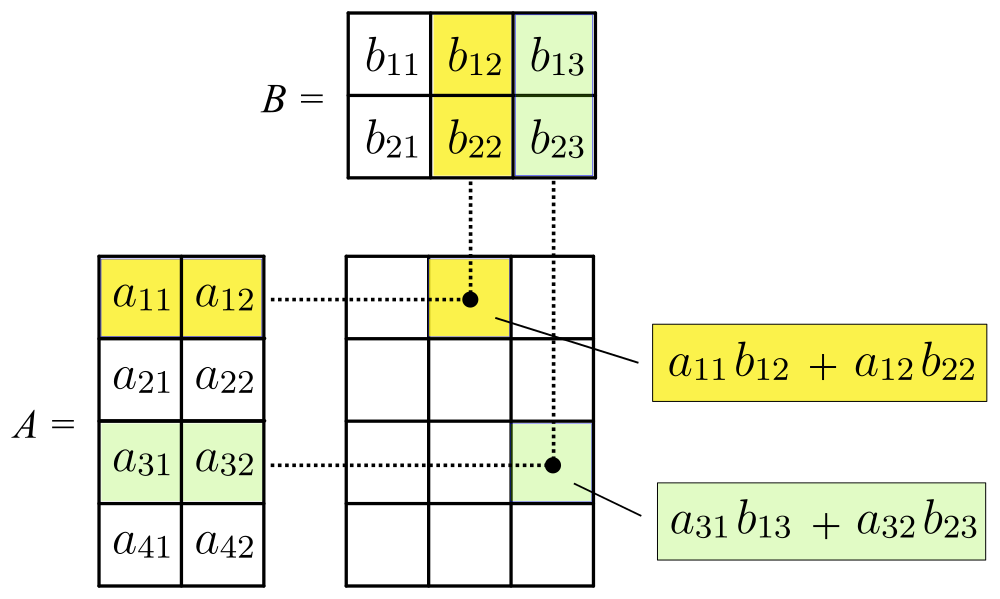
\includegraphics[width=0.35\textwidth]{MatrixMultiplication}

\subsection{Transposition}
$(\mathbf{A}^\mathrm{T})_{i,j}=A_{j,i}$

\section{Special matrices}
\begin{description}
	\item[Square matrix:] The number of rows and columns are the same
	\item[Zero matrix:] All of the elements are zero
	\item[Identity matrix:] A square matrix in which all the elements on the leading diagonal are 1 and the remaining elements are 0, denoted by $\mathbf{I}_k$ for $k\times k$ identity matrix
\end{description}


\section{Determinants}

\subsection{$2\times2$ matrices}
$\begin{vmatrix}a&b\\c&d\end{vmatrix}=ad-bc$

\subsection{$3\times3$ matrices}

$\begin{vmatrix}a&b&c\\d&e&f\\g&h&i\end{vmatrix}=a\begin{vmatrix}e&f\\h&i\end{vmatrix}-b\begin{vmatrix}d&f\\g&i\end{vmatrix}+c\begin{vmatrix}d&e\\g&h\end{vmatrix}=aei+bfg+cdh-ceg-bdi-afh$

\subsection{Singular matrices}
\begin{itemize}
	\item Singular matrices are square matrices with a determinant of 0
	\item It does not have an inverse
	\item If $\mathbf{A}$ and $\mathbf{B}$ are non-singular matrices, then $(\mathbf{AB})^{-1}=\mathbf{B}^{-1}\mathbf{A}^{-1}$
\end{itemize}



\subsection{Properties of determinants}
\begin{itemize}
	\item $\det(\mathbf{AB})=\det(\mathbf{A})\det(\mathbf{B})=\det(\mathbf{B})\det(\mathbf{A})=\det(\mathbf{BA})$
	\item $\det(k\mathbf{A})=k^n\det(\mathbf{A})$ ($\mathbf{A}$ is a $n\times n$ matrix)
\end{itemize}


\section{Inverse matrices}
\subsection{$2\times2$ matrices}
$\begin{bmatrix}
	a & b\\c & d
\end{bmatrix}^{-1}=\dfrac{1}{ad-bc}\begin{bmatrix}
	d & -b\\-c & a
\end{bmatrix}$

\subsection{$3\times3$ matrices}
$\mathbf {A} ^{-1}={\begin{bmatrix}a&b&c\\d&e&f\\g&h&i\\\end{bmatrix}}^{-1}={\frac {1}{\det(\mathbf {A} )}}{\begin{bmatrix}\,A&\,B&\,C\\\,D&\,E&\,F\\\,G&\,H&\,I\\\end{bmatrix}}^{\mathrm {T} }={\frac {1}{\det(\mathbf {A} )}}{\begin{bmatrix}\,A&\,D&\,G\\\,B&\,E&\,H\\\,C&\,F&\,I\\\end{bmatrix}}$\\
$\begin{alignedat}{6}A&={}&(ei-fh),&\quad &D&={}&-(bi-ch),&\quad &G&={}&(bf-ce),\\B&={}&-(di-fg),&\quad &E&={}&(ai-cg),&\quad &H&={}&-(af-cd),\\C&={}&(dh-eg),&\quad &F&={}&-(ah-bg),&\quad &I&={}&(ae-bd).\\\end{alignedat}$

\subsection{Solving equations with matrices}
If $\mathbf{A}\begin{pmatrix}
	x\\y\\z
\end{pmatrix}=\mathbf{v}$ then $\begin{pmatrix}
	x\\y\\z
\end{pmatrix}=\mathbf{A}^{-1}\mathbf{v}$
\begin{description}
	\item[Consistent system of linear equations:] there is at least one set of values that satisfies all the equations simultaneously
	\item[Inconsistent:] such set of values does not exist
\end{description}

\subsection{Possible outcomes of solutions}
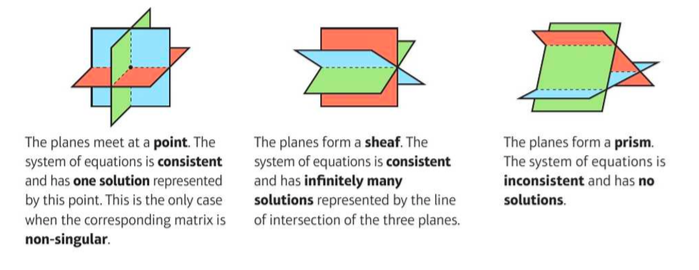
\includegraphics[width=0.75\textwidth]{equations}\\
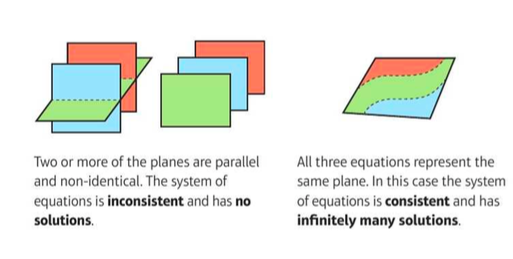
\includegraphics[width=0.5\textwidth]{equations2}

\chapter{Algebraic methods}
\section{Linear transformations in 2D}
\subsection{Properties}
If $L(\vec{v})$ is linear:
\begin{enumerate}
	\item $L(\vec{v})$ should always map the origin onto itself
	\item $L(\vec{v})$ can be represented by a matrix
	\item $L(\vec{v_1}+\vec{v_2})=L(\vec{v_1})+L(\vec{v_2})$ (closure in addition)
	\item $L(\lambda\vec{v_1})=\lambda L(\vec{v_1})$ (closure in scalar multiplication)
\end{enumerate}
\subsection{Invariant points and lines}
\begin{description}
	\item[Invariant points:] Points which are mapped onto themselves under the given transformation
	\item[Invariant lines:] Lines which map onto themselves
\end{description}

\subsection{Reflection}
\begin{description}
	\item[Reflection in $y$-axis:] $\begin{pmatrix}
		-1&0\\0&1
	\end{pmatrix}$, invariant points: points on the $y$-axis; invariant lines: $x=0$, $y=k$
	\item[Reflection in $x$-axis:] $\begin{pmatrix}
		1&0\\0&-1
	\end{pmatrix}$, invariant points: points on the $x$-axis; invariant lines: $y=0$, $x=k$
	\item[Reflection in line $y=x$:] $\begin{pmatrix}
		0&1\\1&0
	\end{pmatrix}$, invariant points: points on $y=x$; invariant lines: $y=x$, $y=-x+k$
	\item[Reflection in line $y=-x$:] $\begin{pmatrix}
		0&-1\\-1&0
	\end{pmatrix}$, invariant points: points on $y=-x$; invariant lines: $y=-x$, $y=x+k$
\end{description}

\subsection{Rotation}
\begin{description}
	\item[Rotation through angle $\theta$ anticlockwise about the origin] $\begin{pmatrix}
		\cos\theta&-\sin\theta\\\sin\theta&\cos\theta
	\end{pmatrix}$
	\item[Invariant points:] Only $(0,0)$
	\item[Invariant lines:] When $\theta=180\textdegree$ any line passing through the origin is an invariant line, otherwise no invariant lines
\end{description}

\subsection{Enlargement / stretches}
\begin{description}
	\item[Transformation matrix] $\begin{pmatrix}
		a & 0 \\ 0 & b
	\end{pmatrix}$ = a stretch of scale factor $a$ parallel to the $x$-axis and scale factor $b$ parallel to the $y$-axis
	\item[Invariant lines] $x$- and $y$-axes for all stretches
	\begin{itemize}
		\item Stretch parallel to the $x$-axes: any line parallel to the $x$-axes
		\item Stretch parallel to the $y$-axes: any line parallel to the $y$-axes
	\end{itemize}
	\item[Invariant points] The origin is always an invariant point
	\begin{itemize}
		\item Stretch parallel to the $x$-axes: points on the $y$-axes
		\item Stretch parallel to the $y$-axes: points on the $x$-axes
	\end{itemize}
	\item[Change in area] $\det(\mathbf{M}) = \text{area scale factor}$
\end{description}

\section{Linear transformations in 3D}
\begin{description}
	\item[Reflection in plane $x=0$] $\begin{pmatrix}
		-1 & 0 & 0\\
		0 & 1 & 0 \\
		0 & 0 & 1
	\end{pmatrix}$
	\item[Reflection in plane $y=0$] $\begin{pmatrix}
		1 & 0 & 0\\
		0 & -1 & 0 \\
		0 & 0 & 1
	\end{pmatrix}$
	\item[Reflection in plane $z=0$] $\begin{pmatrix}
		1 & 0 & 0\\
		0 & 1 & 0 \\
		0 & 0 & -1
	\end{pmatrix}$
	\item[Rotation angle $\theta$ anticlockwise about the $x$-axis] $\begin{pmatrix}
		1 & 0 & 0\\
		0 & \cos\theta & -\sin\theta \\
		0 & \sin\theta & \cos\theta
	\end{pmatrix}$
	\item[Rotation angle $\theta$ anticlockwise about the $y$-axis] $\begin{pmatrix}
	\cos\theta & 0 & \sin\theta \\
	0 & 1 & 0\\
	-\sin\theta & 0 & \cos\theta
	\end{pmatrix}$
	\item[Rotation angle $\theta$ anticlockwise about the $z$-axis] $\begin{pmatrix}
		\cos\theta & -\sin\theta & 0\\
		\sin\theta & \cos\theta & 0\\
		0 & 0 & 1
	\end{pmatrix}$
\end{description}






\chapter{The binomial expansion}
\section{Hyperbolic function definitions}
\subsection{$\sinh x$}
\begin{description}
	\item[Definition] $\sinh x = \dfrac{e^x-e^{-x}}{2}$
	\item[Domain] $x \in \textbf{R}$
	\item[Asymptotes] $x\rightarrow +\infty$, $y\rightarrow\dfrac{e^x}{2}$; $x\rightarrow -\infty$, $y\rightarrow -\dfrac{e^{-x}}{2}$
	\item[x-intercept] $(0,0)$
	\item[y-intercept] $(0,0)$
	\item[Graph]
\end{description}

\subsection{$\cosh x$}
\begin{description}
	\item[Definition] $\cosh x = \dfrac{e^x+e^{-x}}{2}$
	\item[Domain] $x \in \textbf{R}$
	\item[Asymptotes] $x\rightarrow +\infty$, $y\rightarrow\dfrac{e^x}{2}$; $x\rightarrow -\infty$, $y\rightarrow\dfrac{e^{-x}}{2}$
	\item[x-intercept] No
	\item[y-intercept] $(0,1)$
	\item[Graph]
\end{description}

\subsection{$\tanh x$}
\begin{description}
	\item[Definition] $\tanh x = \dfrac{\sinh x}{\cosh x}=\dfrac{e^x-e^{-x}}{e^x+e^{-x}}$
	\item[Domain] $x \in \textbf{R}$
	\item[Asymptotes] $x\rightarrow +\infty$, $y\rightarrow 1$; $x\rightarrow -\infty$, $y\rightarrow -1$
	\item[x-intercept] $(0,0)$
	\item[y-intercept] $(0,0)$
	\item[Graph]
\end{description}

\subsection{$\csch x$}
\begin{description}
	\item[Definition] $\csch x = \dfrac{1}{\sinh x}$
	\item[Domain] 
	\item[Asymptotes] 
	\item[x-intercept] 
	\item[y-intercept] 
	\item[Graph]
\end{description}


\subsection{$\sech x$}
\begin{description}
	\item[Definition] $\sech x = \dfrac{1}{\cosh x}$
	\item[Domain] 
	\item[Asymptotes] 
	\item[x-intercept] 
	\item[y-intercept] 
	\item[Graph]
\end{description}


\subsection{$\coth x$}
\begin{description}
	\item[Definition] $\coth x = \dfrac{\cosh x}{\sinh x}$
	\item[Domain] 
	\item[Asymptotes] 
	\item[x-intercept] 
	\item[y-intercept] 
	\item[Graph]
\end{description}

\section{Identities of hyperbolic functions}
Similar to trigonometric identities:
\begin{itemize}
	\item $\tanh x = \dfrac{\sinh x}{\cosh x}$
	\item $\cosh^2 x - \sinh^2 x = 1$
	\item $\tanh^2 x + \sech^2 x= 1$
	\item $\coth^2 x - \csch^2 x = 1$
\end{itemize}

\subsection{Addition}
\begin{itemize}
	\item $\sinh(x+y)=\sinh x \cosh y + \sinh y \cosh x$
	\item $\cosh(x+y)=\cosh x \cosh y + \sinh x \sinh y$
	\item $\tanh(x+y) = \dfrac{\sinh(x+y)}{\cosh(x+y)} = \dfrac{\sinh x \cosh y + \sinh y \cosh x}{\cosh x \cosh y + \sinh x \sinh y} = \dfrac{\frac{\sinh x}{\cosh x}+\frac{\sinh y}{\cosh y}}{1 + \frac{\sinh x \sinh y}{\cosh x \cosh y}}=\dfrac{\tanh x + \tanh y}{1 + \tanh x \tanh y}$
\end{itemize}

\subsection{Double angle}
\begin{itemize}
	\item $\sinh 2x = 2\sinh x \cosh x$
	\item $\cosh 2x = \cosh^2 x + \sinh^2 x = 2\cosh^2 x - 1 = 2\sinh^2 + 1$
	\item $\tanh 2x = \dfrac{2\tanh x}{1 + \tanh^2 x}$
\end{itemize}

\subsection{Power descending}


\section{Differentiating hyperbolic functions}
\begin{itemize}
	\item $(\sinh x)'=\cosh x$
	\item $(\cosh x)'=\sinh x$
	\item $(\tanh x)'=1-\tanh^2 x = \sech^2 x$
	\item $(\csch x)'=-\coth x \csch x$
	\item $(\sech x)'=-\sech x \tanh x$
	\item $(\coth x)'=-\sech^2 x$
\end{itemize}

\chapter{Trigonometric ratios}
\section{SUVAT equations}
\begin{itemize}
    \item $s=ut+\dfrac{1}{2}at^2$
    \item $s=vt-\dfrac{1}{2}at^2$
    \item $v=u+at$
    \item $v^2=u^2+2as$
    \item $s=\dfrac{1}{2}(u+v)t$
\end{itemize}


\chapter{Trigonometric identities and equations}
\section{Types of forces}
\begin{description}
    \item[Weight:] $W=mg$
    \item[Normal contact force:] symbol = $R$ or $N$
    \item[Static friction:] Depends on driving force, $F\leq \mu R$
    \item[Dynamic friction:] $f=\mu R$ ($\mu$=coefficient of kinetic friction), exists on \textbf{rough surfaces}
    \item[Thrust / compression:] Object being pushed along using a light rod
    \item[Tension:] $T=\text{elastic coefficient}\times\text{extension}=k\times\Delta x$
    \item[Air resistance / drag:] resistance due to air / water / fluid
    \item[Driving / propulsive force:] forward force produced by the object itself
\end{description}

\section{Common scenarios}
\subsection{Connected particles}
\begin{itemize}
    \item Acceleration is the same across the whole system
    \item Internal force can be ignored
    \item Tension at the same rope has the same magnitude
\end{itemize}

\subsection{Lift}
\begin{itemize}
    \item Consider the whole system to find tension in the string
    \item Consider one object only to find force they exerted on each other
    \item Rising: $R-W=ma$
    \item Moving down: $W-R=ma$
    \item On rest: $R=W$
\end{itemize}

\subsection{Fixed pulley}
\begin{itemize}
    \item Same tension
    \item Same magnitude for acceleration (different direction)
    \item Use simultaneous equations to find tension
    \item $\text{Force on pulley} = 2 \times \text{tension}$
\end{itemize}

\chapter{Vectors}
\section{Definition}
$\int_{a}^{b} f(x) \: dx = \lim\limits_{\delta x\rightarrow0}\sum_{x=a}^{b}f(x)\delta x$

\section{Formulae}
\subsection{Integrating trigonometric functions}
\begin{itemize}
    \item $\int\sin x \dx = -\cos x + c$
    \item $\int\cos x \dx = \sin x + c$
    \item $\int \tan x \dx = -\ln |\cos x| + c= \ln |\sec x| + c$
    \item $\int \cot x \dx = \ln |\sin x| + c = -\ln |\csc x| + c$
    \item $\int \sec x \dx = \int \frac{\sec x(\sec x + \tan x)}{\sec x + \tan x} \dx = \ln |\sec x + \tan x| + c = \ln \left|\tan\left(\frac{1}{2}x+\frac{1}{4}\pi \right)\right| + c$
    \item $\int \csc x \dx = -\ln|\csc x + \cot x| + c = \ln \left|\tan\left(\frac{1}{2}x\right)\right| + c$
    \item $\int \sin^2 x \dx = \int \frac{1-\cos 2x}{2} \dx = \frac{2x-\sin 2x}{4} + c$
    \item $\int \cos^2 x \dx = \int \frac{1+\cos 2x}{2} \dx = \frac{2x+\sin 2x}{4} + c$
    \item $\int \tan^2 x \dx = \int \sec^2 x -1 \dx = \tan x - x + c$
    \item $\int \cot^2 x \dx = \int \csc^2 x -1 \dx = -\cot x - x + c$
    \item $\int \sin x \cos x \dx = \int \frac{\sin 2x}{2} \dx = -\frac{\cos 2x}{4} + c$
    \item $\int \tan x \sec x \dx = \sec x + c$
    \item $\int \cot x \csc x \dx = -\csc x + c$
\end{itemize}
Integrating $\sin^2x$ or $\cos^2x$ (power descending):
\begin{itemize}
    \item $\int \sin ^2 x \: dx=\int \frac{1-\cos 2x}{2} \: dx=\frac{1}{2}\left(x-\frac{\sin 2x}{2}\right)+c$
    \item $\int \cos ^2 x \: dx=\int \frac{1+\cos 2x}{2} \: dx= \frac{1}{2}\left(x+\frac{\sin 2x}{2}\right)+c$
\end{itemize}
By part:
\begin{itemize}
    \item $\int \ln x \: dx = x\ln x + x + c$
\end{itemize}
\section{Techniques}
\subsection{U-sub}
\begin{itemize}
    \item $\int f'(ax+b) \: dx = \frac{f(ax+b)}{a}+c$
          \begin{description}
              \item[Substitution:] $u=ax+b$
          \end{description}
    \item $\int \frac{f'(x)}{f(x)} \: dx = \ln |f(x)|+c$
          \begin{description}
              \item[Substitution:] $u=f(x)$
          \end{description}
\end{itemize}
\subsection{By part}
\begin{itemize}
    \item $\int u \: dv = uv - \int v \: du$
    \item LIPET rule: leftmost = $u$
        \begin{description}
            \item[L:] logarithmic
            \item[I:] inverse trigonometry
            \item[P:] polynomial
            \item[E:] exponential
            \item[T:] trigonometry
        \end{description}
\end{itemize}

\chapter{Differentiation}
\section{The first principle}
$$f'(x) = \lim\limits_{n \to 0}\dfrac{f(x+h)-f(x)}{h}$$


\chapter{Integration}
\input{chapters/P1/13.tex}

\chapter{Exponentials and logarithms}
\section{Sketching graphs}
Find the y-intercept of the graph

\section{$e^x$ function}
\begin{description}
    \item $(e^x)'$ = $e^x$ (gradient = $y$ value)
    \item $(e^{kx})'$ = $ke^{kx}$ (gradient directly proportional to $y$ value)
\end{description}

\section{Logarithm}
$a^x = n$: $\log_a n = x$ ($a\neq1$ and $a>0$, $x>0$)
\subsection{Laws}
\begin{description}
    \item[The multiplication law:] $\log_a x + \log_a y = \log_a xy$
    \item[The division law:] $\log_a x - \log_a y = \log_a\left(\dfrac{x}{y}\right)$
    \item[The power law:] $\log_a x^k = k\log_a x$
    \item[Change base formula]: $\log_a b = \dfrac{\log_c b}{\log_c a}$
\end{description}

\subsection{Logarithms in non-linear form}
\textbf{Exponential}
\begin{itemize}
    \item $y=ab^x\rightarrow\ln y = x\ln b + \ln a$
    \item x-axis = $x$, y-axis = $\ln y$, gradient = $\ln b$, y-intercept = $\ln a$
\end{itemize}
\textbf{Power}
\begin{itemize}
    \item $y=ax^b\rightarrow\ln y = b\ln x + \ln a$
    \item x-axis = $\ln x$, y-axis = $\ln y$, gradient = $b$, y-intercept = $\ln a$
\end{itemize}
\textbf{Logarithmic}
\begin{itemize}
    \item $y=a\ln x\rightarrow$ kept the same
    \item x-axis = $\ln x$, y-axis = $y$, gradient = $a$
\end{itemize}

\part{Pure 2 Contents}
\chapter{Algebraic methods}
\section{Proof by contradiction}
\subsection{Steps}
\begin{enumerate}
    \item Assume that the first statement is false
    \item Use logical steps / contradiction from knowledge to show that the assumption is false
    \item Conclude that the assumption is false so the original statement must be true
\end{enumerate}
\subsection{Irrationality of $\sqrt{2}$}
\begin{description}
    \item [Assumption:] $\sqrt{2}$ is a rational number
    \item Then $\sqrt{2} = \dfrac{a}{b}$ for some integers $a$ and $b$
    \item Also assume that $a$ and $b$ has no common factors so the fraction is in the simplest form
    \item So $2=\dfrac{a^2}{b^2}$, $a^2=2b^2$
    \item So $a^2$ must be even, so a is also even
    \item If $a$ is even, then it can be expressed in the form $a=2n$, where $n$ is an integer
    \item Substitute $a=2n$: $(2n)^2=2b^2$
    \item So $4n^2 = 2b^2$
    \item So $b^2=2n^2$, hence $b^2$ must be even and b is also even
    \item If $a$ and $b$ are both even, they will have a common factor or 2
    \item This contradicts that $a$ and $b$ has no common factors, so $\sqrt{2}$ is an irrational number
\end{description}


\subsection{Infinity of primes}
\begin{description}
    \item [Assumption:] there is a finite number of prime numbers
    \item List all the prime numbers that exist: $p_1, p_2, p_3, \dots, p_n$
    \item Consider the number $N = p_1 \times p_2 \times p_3 \times \dots \times p_n + 1$
    \item When $N$ is divided by any of $p_1, p_2, p_3, \dots, p_n$ a remainder of $1$ is produced so none of them is a factor of $N$
    \item Therefore $N$ must be prime or have a prime factor not in the list of all the prime numbers that exist
    \item This contradicts the assumption that there is a finite number of prime numbers
    \item Therefore there must be an infinite number of prime numbers
\end{description}


\chapter{Functions and graphs}
\section{Maclaurin series}
$$f(x)=f(0)+f'(0)x+\frac{f''(0)x^2}{2!}+\dots+\frac{f^{(r)}(0)x^r}{r!}+\dots$$
This series is valid provided that $f(0), f'(0), f''(0),\dots,f^{(r)}(0),\dots$ all have \textbf{finite values}

\section{Series expansion of compound functions}
\begin{itemize}
    \item $e^{x}=1+x+\frac{x^{2}}{2!}+...+\frac{x^{r}}{r!}+...$ for all $x$
    \item $\ln(1+x) = x - \frac{x^{2}}{2} + \frac{x^{3}}{3} + ... + (-1)^{r+1}\frac{x^{r}}{r!} +...$ for $-1<x\leq1$
    \item $\sin x = \frac{e^{ix}-e^{-ix}}{2i}=x-\frac{x^{3}}{3!}+\frac{x^{5}}{5!}+...+(-1)^r\dfrac{x^{2r+1}}{(2r+1)!}+\dots$ for all $x$
    \item $\cos x = \frac{e^{ix}+e^{-ix}}{2}=1-\frac{x^{2}}{2!}+\frac{x^{4}}{4!}-...+(-1)^r\dfrac{x^{2r}}{(2r)!}+\dots$ for all $x$
    \item $\arctan x = x-\dfrac{x^3}{x}+\dfrac{x^5}{5}-\dots+(-1)^r\dfrac{x^{2r+1}}{2r+1}+\dots$ for $-1<x\leq1$
\end{itemize}

\section{Proving series properties}
\begin{enumerate}
    \item Use Taylor and Maclaurin Series
    \item Use basic formulae for expansion
    \item Use geometric series
\end{enumerate}

\section{Testing for convergence}
\subsection{$n$th term test}
\begin{itemize}
    \item $\lim_{n\rightarrow\infty}a_n \neq 0$ $\rightarrow$ $\sum_{n=1}^{\infty}a_n$ diverges
    \item $\sum_{n=1}^{\infty}a_n$ converges $\rightarrow$ $\lim_{n\rightarrow\infty}a_n = 0$
\end{itemize}

\subsection{Integral test}
\begin{itemize}
    \item If $a_n$ decrease and $a_n>0$, $\sum_{n=1}^{\infty}a_n$ and $\int_{1}^{\infty} f(x) \dx$
          has the same properties of convergence or divergence
\end{itemize}

\subsection{Comparison test}
Suppose $b_n<a_n$ for all $n$:
\begin{itemize}
    \item $\sum_{n=1}^{\infty}b_n$ diverges $\rightarrow$ $\sum_{n=1}^{\infty}a_n$ diverges
    \item \item $\sum_{n=1}^{\infty}a_n$ converges $\rightarrow$ $\sum_{n=1}^{\infty}b_n$ converges
    \item Compare $a_n$ with $p$-series and geometrical series
          \begin{description}
              \item[$p$-series] $\sum_{n=1}^{\infty} \left(\frac{1}{n}\right)^p$ is divergent if $p\leq 1$ and
                    convergent if $p>1$
          \end{description}
\end{itemize}

\subsection{Root test}
\begin{itemize}
    \item $\lim_{n\rightarrow\infty}\sqrt[n]{a_n} < 1$ $\rightarrow$ $a_n$ converge
    \item \item $\lim_{n\rightarrow\infty}\sqrt[n]{a_n} > 1$ $\rightarrow$ $a_n$ diverge
\end{itemize}

\subsection{Ratio test}
\begin{itemize}
    \item $\lim_{n\rightarrow\infty} \left|\frac{a_{n+1}}{a_n}\right| < 1$: convergent
    \item $\lim_{n\rightarrow\infty} \left|\frac{a_{n+1}}{a_n}\right| > 1$: divergent
    \item $\lim_{n\rightarrow\infty} \left|\frac{a_{n+1}}{a_n}\right| = 1$: not sure
\end{itemize}

\section{Summation of series}
\begin{itemize}
    \item Try to break down $a_n$ into the form $a_n=b_{n+1}-b_n$
\end{itemize}

\chapter{Sequences and series}
\section{Divergent / convergent series}
$\sum\limits_{i=1}^{n} u_i = u_1+u_2+u_3+\dots+u_n$\\
If $\lim\limits_{n \to \infty}S_n$ exists, $\sum\limits_{i=1}^{n} u_i$ converges\\
If $\lim\limits_{n \to \infty}S_n$ does not exist, $\sum\limits_{i=1}^{n} u_i$ diverges
\section{Geometric series}
\begin{description}
    \item [Sum of first n terms:]$S_n = \dfrac{a(1-r^n)}{1-r}$
    \item [Sum to infinity:] When $|r|<1$ (convergent series): $S_\infty = \dfrac{a}{1-r}$
\end{description}

\section{Recurrence relations}
\begin{description}
    \item[Increasing sequence:] $u_{n+1}>u_n$ for all $n\in \mathbf{N}$
    \item[Decreasing sequence:] $u_{n+1}<u_n$ for all $n\in \mathbf{N}$
    \item[Periodic sequence:] If there is an integer $k$ such that $u_{n+k}=u_n$ for all $n\in \mathbf{N}$, $k$ = the order of the sequence
\end{description}

\chapter{Binomial expansion}
\section{Binomial expansion}
* Always write the answer in \textbf{ascending} powers of $x$
\subsection{Expanding $(1+x)^n$}
When $|x|<1$:\\
$(1+x)^n\approx 1 + nx + \dfrac{n(n-1)}{2!}x^2+\dfrac{n(n-1)(n-2)}{3!}x^3+\dots$
\subsection{Expanding $(a+bx)^n$}
$(a+bx)^n = \left(a\left(1+\dfrac{b}{a}x\right)\right)^n = a^n\left(1+\dfrac{b}{a}x\right)^n$\\
Valid for $\left|\dfrac{b}{a}x\right|<1$ or $|x| < \dfrac{a}{b}$

\chapter{Radians}
\section{Radians calculations}
\begin{description}
    \item[Arc length] $s=r\theta$
    \item[Area of sector] $A=\dfrac{1}{2}r^2\theta$
\end{description}

\section{Small angle approximation}
When $\theta$ is small:
\begin{itemize}
    \item $\sin \theta \approx \theta$
    \item $\cos \theta \approx 1-\dfrac{\theta^2}{2}$
    \item $\tan \theta \approx \theta$
\end{itemize}


\chapter{Trigonometric functions}
\section{Identities}
\begin{itemize}
    \item $\tan \theta = \dfrac{\sin \theta}{\cos \theta}$
    \item $\sin^2 \theta + \cos^2 \theta = 1$
    \item $\tan^2 \theta + 1 = \sec^2 \theta$
    \item $\cot^2 \theta + 1 = \cosec^2 \theta$
\end{itemize}

\section{secant, cosecant and cotangent}
\subsection{Graphs}
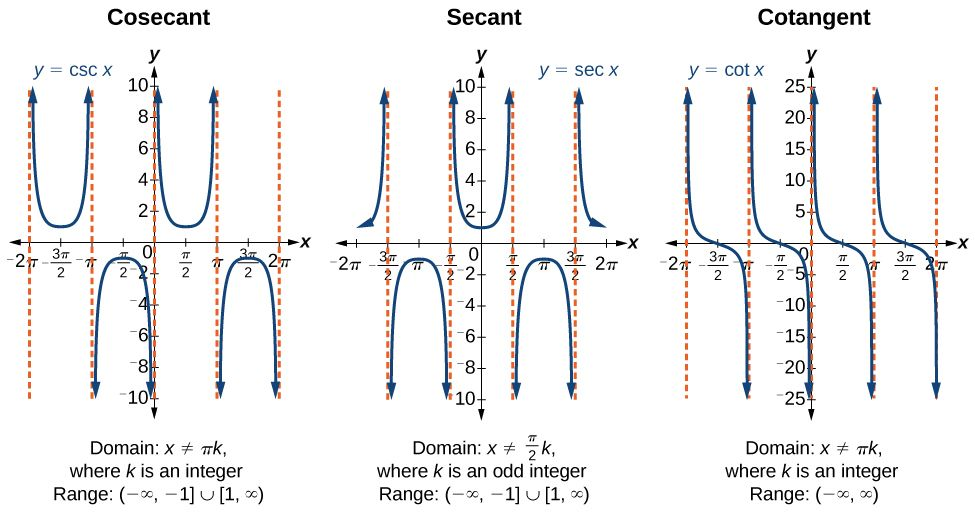
\includegraphics[scale=0.9]{csc-sec-cot-graphs}

\subsection{Identities}
\begin{itemize}
    \item $\tan \theta = \dfrac{\sin \theta}{\cos \theta}$
    \item $\sin^2 \theta + \cos^2 \theta = 1$
    \item $\tan^2 \theta + 1 = \sec^2 \theta$
    \item $\cot^2 \theta + 1 = \cosec^2 \theta$
\end{itemize}

\section{arcsin, arccos, arctan}
\subsection{Graphs}
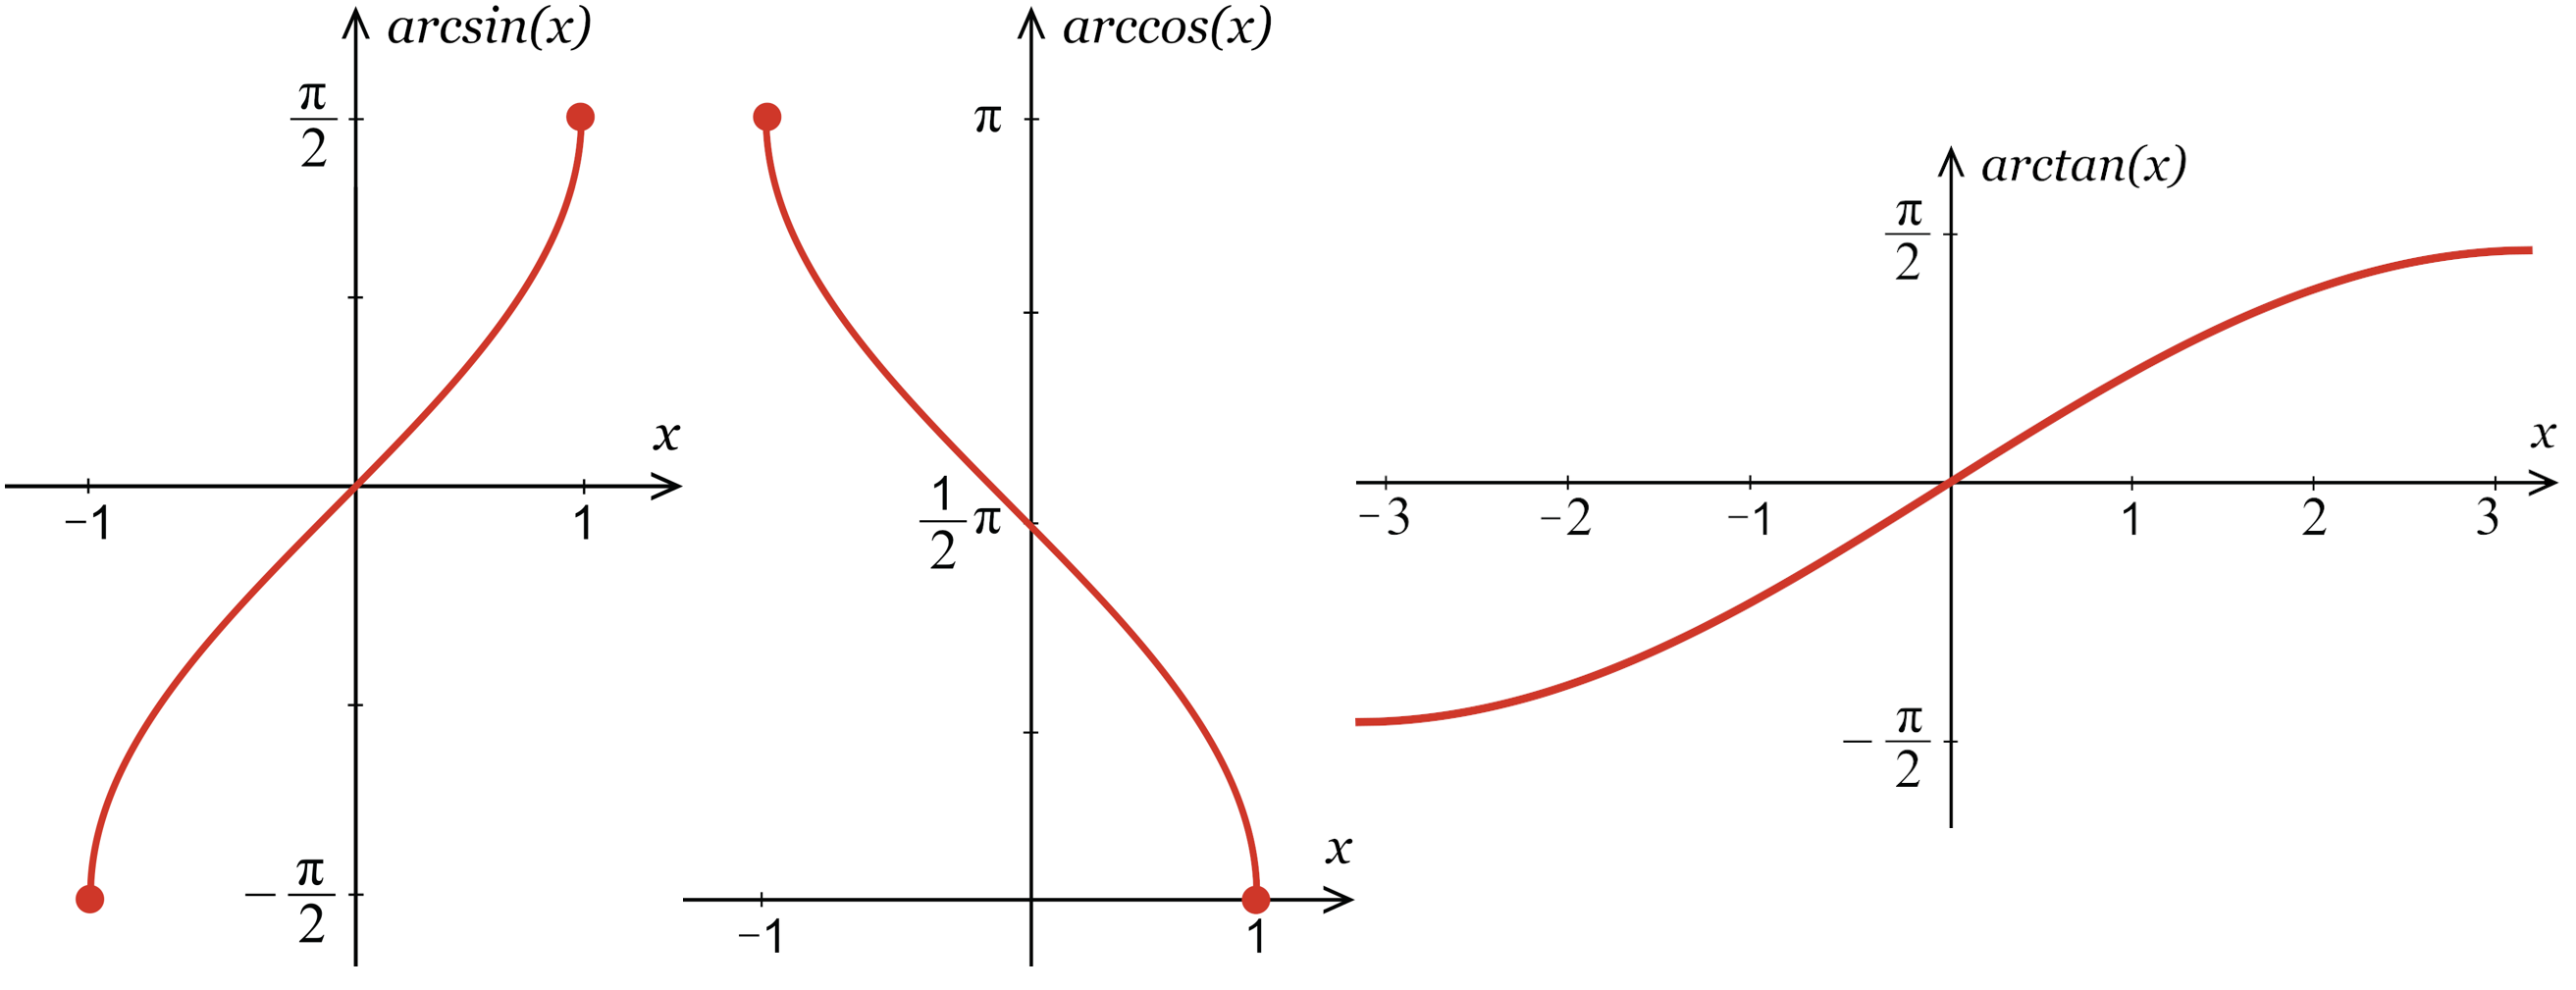
\includegraphics[scale=0.7]{arcsincostan}



\chapter{Trigonometry and modelling}
\section{Trigonometry formulae}
\subsection{Addition / subtraction}
\begin{itemize}
    \item $\sin (A \pm B) = \sin A \cos B \pm \cos A \sin B$
    \item $\cos (A \pm B) = \cos A \cos B \mp \sin A \sin B$
    \item $\tan (A \pm B) = \dfrac{\tan A \pm \tan B}{1 \mp \tan A \tan B}$
\end{itemize}
\subsection{Sum to product identities}
\begin{itemize}
    \item $\sin A + \sin B = 2\sin \dfrac{A+B}{2} \cos\dfrac{A-B}{2}$
    \item $\sin A - \sin B = 2\cos \dfrac{A+B}{2} \sin\dfrac{A-B}{2}$
    \item $\cos A + \cos B = 2\cos \dfrac{A+B}{2} \cos\dfrac{A-B}{2}$
    \item $\cos A - \cos B = -2\sin \dfrac{A+B}{2} \sin\dfrac{A-B}{2}$
\end{itemize}
\subsection{Double angle}
\begin{itemize}
    \item $\sin 2A = 2\sin A \cos A$
    \item $\cos 2A = \cos^2 A - \sin^2 A$
    \item $\tan 2A = \dfrac{2\tan A}{1-\tan^2 A}$
\end{itemize}
\subsection{Power descending}
(Derive from double angle)
\begin{itemize}
    \item $\sin A \cos A = \dfrac{\sin2A}{2}$
    \item $\sin^2 A = \dfrac{1-\cos2A}{2}$
    \item $\cos^2 A = \dfrac{1+\cos2A}{2}$
\end{itemize}
\subsection{Half angle}
\begin{itemize}
    \item $\sin \dfrac{A}{2} = \pm \sqrt{\dfrac{1-\cos A}{2}}$
    \item $\cos \dfrac{A}{2} = \pm \sqrt{\dfrac{1+\cos A}{2}}$
    \item $\tan \dfrac{A}{2} = \pm \sqrt{\dfrac{1-\cos A}{1+\cos A}} = \dfrac{1-\cos A}{\sin A} = \dfrac{\sin A}{1+\cos A}$
\end{itemize}

\section{Trigonometric equations}
\subsection{Principal values}
The angle that you get when you use the inverse trigonometric functions on the calculator
\begin{itemize}
    \item $\sin^{-1}$: $-\dfrac{\pi}{2}\leq\theta\leq\dfrac{\pi}{2}$
    \item $\cos^{-1}$: $0\leq\theta\leq\pi$
    \item $\tan^{-1}$: $-\dfrac{\pi}{2}\leq\theta\leq\dfrac{\pi}{2}$
\end{itemize}

\chapter{Parametric equations}
\section{Converting to Cartesian form}
\begin{itemize}
    \item Express $t$ in terms of $x$, then substitute $t=f(x)$ into $y=g(t)$
    \item Find the range of $x$ by using the original parametric equation
    \item Find the range of $y$ using original equation / considering the domain of $x$
\end{itemize}
\section{Sketching curves}
\begin{itemize}
    \item Sketch at regular intervals of $t$
\end{itemize}

\chapter{Differentiation}
\section{Proving differentiation formulae}
\subsection{$\sin x$ and $\cos x$}
Use the fact that when $h\rightarrow0$, $\lim_{h\rightarrow0} \frac{\sin h}{h} = 1$ 
and $\lim_{h\rightarrow0} \frac{\cos h - 1}{h} = 0$

\section{Formulae for trigonometric functions}
\begin{itemize}
    \item $(\tan kx)' = k\sec^2 kx$
    \item $(\sec kx)' = k\sec kx \tan kx$
    \item $(\cot kx)' = -k\csc^2 kx$
    \item $(\csc kx)' = -k\csc kx \cot kx$
\end{itemize}

\section{Rules}
\begin{description}
    \item[Chain rule:] $\dfrac{dy}{dx} = \dfrac{dy}{du} \times \dfrac{du}{dx}$
    \item[Product rule:] $(f(x)g(x))'=f'(x)g(x)+g'(x)f(x)$
    \item[Quotient rule:] $\dfrac{f(x)}{g(x)} = \dfrac{f'(x)g(x)-g'(x)f(x)}{g^2(x)}$
\end{description}


\section{Tangent and normal}
For curve $y=f(x)$:
\begin{description}
    \item[Tangent at $(a,f(a))$:] $y-f(a)=f'(a)(x-a)$
    \item[Normal at $(a,f(a))$:] $y-f(a)=-\dfrac{1}{f'(a)}(x-a)$
\end{description}

\chapter{Numerical methods}
\section{Locating roots}
\subsection{Method}
If a function $f(x)$ is continuous on the interval $[a,b]$ and $f(a)$ and $f(b)$ have opposite signs, then $f(x)$ has at least one root, $x$, which satisfies $a<x<b$
\subsection{How change of sign can fail}
\begin{itemize}
    \item When the interval is too large sign may not change as there may be an even number of roots
    \item If the function is not continuous, sign may change but there may be an asymptote e.g. reciprocal
\end{itemize}

\section{Iteration}
\begin{itemize}
    \item Iterative formula can be found by rewriting $f(x)=0$ into $x=g(x)$, then $x_{n+1}=g(x_n)$
    \item Find the value of $x_1$, $x_2$, $x_3$, etc.
    \item If converge (get closer to the root from the same direction / alternate above and below the root) then solution can be found
    \item Test for roots using the change of sign of function $h(x)=g(x)-x$
\end{itemize}

\section{The Newton-Raphson method}
\begin{itemize}
    \item $x_{n+1}=x_n-\dfrac{f(x_n)}{f'(x_n)}$
    \item Find approximation to $x$ decimal places
    \item Show accurate to $x$ decimal places: use change in sign to show
    \item[$\star$] If any value of $x_i$ is at a turning point then the method will fail as $f'(x)=0$ which results in division by zero
\end{itemize}

\section{The trapezium rule}
$\int_{a}^{b}y\:dx \approx \dfrac{1}{2} h (y_0+2(y_1+y_2+\dots+y_{n-1})+y_n)$ where $h=\dfrac{b-a}{n}$ and $y_i=f(a+ih)$


\chapter{Integration}
\section{Definition}
$\int_{a}^{b} f(x) \: dx = \lim\limits_{\delta x\rightarrow0}\sum_{x=a}^{b}f(x)\delta x$

\section{Formulae}
\subsection{Integrating trigonometric functions}
\begin{itemize}
    \item $\int\sin x \dx = -\cos x + c$
    \item $\int\cos x \dx = \sin x + c$
    \item $\int \tan x \dx = -\ln |\cos x| + c= \ln |\sec x| + c$
    \item $\int \cot x \dx = \ln |\sin x| + c = -\ln |\csc x| + c$
    \item $\int \sec x \dx = \int \frac{\sec x(\sec x + \tan x)}{\sec x + \tan x} \dx = \ln |\sec x + \tan x| + c = \ln \left|\tan\left(\frac{1}{2}x+\frac{1}{4}\pi \right)\right| + c$
    \item $\int \csc x \dx = -\ln|\csc x + \cot x| + c = \ln \left|\tan\left(\frac{1}{2}x\right)\right| + c$
    \item $\int \sin^2 x \dx = \int \frac{1-\cos 2x}{2} \dx = \frac{2x-\sin 2x}{4} + c$
    \item $\int \cos^2 x \dx = \int \frac{1+\cos 2x}{2} \dx = \frac{2x+\sin 2x}{4} + c$
    \item $\int \tan^2 x \dx = \int \sec^2 x -1 \dx = \tan x - x + c$
    \item $\int \cot^2 x \dx = \int \csc^2 x -1 \dx = -\cot x - x + c$
    \item $\int \sin x \cos x \dx = \int \frac{\sin 2x}{2} \dx = -\dfrac{\cos 2x}{4} + c$
    \item $\int \tan x \sec x \dx = \sec x + c$
    \item $\int \cot x \csc x \dx = -\csc x + c$
\end{itemize}
Integrating $\sin^2x$ or $\cos^2x$ (power descending):
\begin{itemize}
    \item $\int \sin ^2 x \: dx=\int \dfrac{1-\cos 2x}{2} \: dx=\dfrac{1}{2}\left(x-\dfrac{\sin 2x}{2}\right)+c$
    \item $\int \cos ^2 x \: dx=\int \dfrac{1+\cos 2x}{2} \: dx= \dfrac{1}{2}\left(x+\dfrac{\sin 2x}{2}\right)+c$
\end{itemize}
By part:
\begin{itemize}
    \item $\int \ln x \: dx = x\ln x + x + c$
\end{itemize}
\section{Techniques}
\subsection{U-sub}
\begin{itemize}
    \item $\int f'(ax+b) \: dx = \dfrac{f(ax+b)}{a}+c$
          \begin{description}
              \item[Substitution:] $u=ax+b$
          \end{description}
    \item $\int \dfrac{f'(x)}{f(x)} \: dx = \ln |f(x)|+c$
          \begin{description}
              \item[Substitution:] $u=f(x)$
          \end{description}
\end{itemize}
\subsection{By part}
\begin{itemize}
    \item $\int u \: dv = uv - \int v \: du$
    \item LIPET rule: leftmost = $u$
        \begin{description}
            \item[L:] logarithmic
            \item[I:] inverse trigonometry
            \item[P:] polynomial
            \item[E:] exponential
            \item[T:] trigonometry
        \end{description}
\end{itemize}

\chapter{Vectors}
\section{Angle with $x$-, $y$-, and $z$-axis (direction cosines)}
If $\vec{a}=x\vec{i}+y\vec{j}+z\vec{k}$ makes an angle $\theta_x$ with the positive x-axis then $\cos \theta_x=\dfrac{x}{|a|}$, similarly for angles $\theta_y$ and $\theta_z$

\section{Vectors in equations}
\subsection{2D}
If $\vec{a}$ and $\vec{b}$ are 2 non-parallel vectors and $p\vec{a}+q\vec{b}=r\vec{a}+s\vec{b}$ then $p=r$ and $q=s$

\subsection{3D}
If $\vec{a}$, $\vec{b}$ and $\vec{c}$ are vectors in 3 dimensions which do not all lie on the same plane (parallel to the same plane) then you can compare their coefficients on both sides of an equation

\section{Modelling with vectors}
$\star$ Be careful about whether the question asked to use vector or scalar quantities
\subsection{Vector quantities}
\begin{itemize}
    \item $\vec{v}$ = velocity
    \item $\overrightarrow{AB}$ = \textbf{displacement} from $A$ to $B$
\end{itemize}

\subsection{Scalar quantities}
\begin{itemize}
    \item $|\vec{v}|$ = speed
    \item $|\overrightarrow{AB}|$ = \textbf{distance} in a straight line from $A$ to $B$
\end{itemize}

\end{document}